\documentclass{jorbnc_cheatsheet}

\begin{document}

\begin{multicols*}{4}

\parbox{\columnwidth}{\centering\Huge\color{Black}\textbf{SCMx1\strut}}\scriptsize

\sectionbox{Supply Chain Management \& Logistics}

\subsection{Classical Logistics}

\subsubsectionbox{Logistics as "organization of a complex operation"}{}{
}

\subsubsectionbox{Logistics in Manufacturing}{}{
}

\subsubsectionbox{Logistics in Services}{}{
}

\subsection{Supply Chain Management}

\subsubsectionbox{What is a Supply Chain?}{}{
}

\subsubsectionbox{Supply Networks}{}{
\vspace{-2mm}
\begin{figure}[H]
	\centering
	\begin{tikzpicture}
		[node distance=35pt,on grid,
		red, thick,
		every place/.style= {minimum size=2.5mm, draw=BrickRed, fill=BrickRed!70},
		sup place/.style= {place, draw=red, fill=BrickRed!25, thin}, % sup -> supplier
		dis place/.style= {place, draw=blue, fill=darkblue!25, thin}, % dis -> distributor
		every label/.style= {text=red, font=\tiny}
		]
		
		% Focal Company
		\node [place] (M) [minimum size=4mm] {};
		
		% Suppliers
		\node [sup place] (ST1_1) [left=of M, yshift=20pt, minimum size=3mm] {} edge [red, thick] (M);
			\node [sup place] (ST2_1) [left=of ST1_1, yshift=18pt] {} edge [dashed, thin] (ST1_1);
			\node [sup place] (ST2_2) [left=of ST1_1, yshift=9pt] {} edge [] (ST1_1);
			\node [sup place] (ST2_3) [left=of ST1_1, yshift=0pt] {} edge [dashed, thin] (ST1_1);
		\node [sup place] (ST1_2) [left=of M, minimum size=3mm] {} edge [red, thick] (M);
			\node [sup place] (ST2_4) [left=of ST1_2, yshift=9pt] {} edge [dashed, thin] (ST1_2);
			\node [sup place] (ST2_5) [left=of ST1_2, yshift=0pt] {} edge [dashed, thin] (ST1_2);
			\node [sup place] (ST2_6) [left=of ST1_2, yshift=-9pt] {} edge [dashed, thin] (ST1_2);
		\node [sup place] (ST1_3) [left=of M, , yshift=-20pt, minimum size=3mm] {} edge [red, thick] (M);
			\node [sup place] (ST2_7) [left=of ST1_3, yshift=0pt] {} edge [dashed, thin] (ST1_3);
			\node [sup place] (ST2_8) [left=of ST1_3, yshift=-9pt] {} edge [thin, black, dotted] (ST1_3);
			\node [sup place] (ST2_9) [left=of ST1_3, yshift=-18pt] {} edge [thin, black, dotted] (ST1_3);
		
		% Distributors
		\node [dis place] (D1) [right=of M, yshift=20pt, minimum size=3mm] {} edge [blue] (M);
			\node [dis place] (R1) [right=of D1, yshift=18pt] {} edge [blue, dashed, thin] (D1);
			\node [dis place] (R2) [right=of D1, yshift=9pt] {} edge [blue] (D1);
			\node [dis place] (R3) [right=of D1, yshift=0pt] {} edge [blue, dashed, thin] (D1);
		\node [dis place] (D2) [right=of M, minimum size=3mm] {} edge [blue] (M);
			\node [dis place] (R4) [right=of D2, yshift=9pt] {} edge [blue] (D2);
			\node [dis place] (R5) [right=of D2, yshift=0pt] {} edge [blue] (D2);
			\node [dis place] (R6) [right=of D2, yshift=-9pt] {} edge [blue, dashed, thin] (D2);
		\node [dis place] (D3) [right=of M, yshift=-20pt, minimum size=3mm] {} edge [blue] (M);
			\node [dis place] (R7) [right=of D3, yshift=0pt] {} edge [blue, dashed, thin] (D3);
			\node [dis place] (R8) [right=of D3, yshift=-9pt] {} edge [blue] (D3);
			\node [dis place] (R9) [right=of D3, yshift=-18pt] {} edge [blue, dashed, thin] (D3);
		
		% Tier Labels
		\node (L) [above=of M, yshift=5pt, label={[align=left]Focal\\Company}] {};
		\node (L2) [left=of L, label={[align=left]Tier 1\\Suppliers}] {};
		\node (L3) [left=of L2, label={[align=left]Tier 2\\Suppliers}] {};
		\node (L4) [right=of L, label={[align=left,text=blue]Tier 1\\Customers}] {};
		\node (L5) [right=of L4, label={[align=left,text=blue]Tier 2\\Customers}] {};

	\end{tikzpicture}
\end{figure}
In a manufacturing context, a supply chain can be seen as a network of suppliers, manufacturers, distributors, and retailers.
}

\subsubsectionbox{SCM vs. Logistics}{}{
}

\subsubsectionbox{SCM Cycles}{}{
}

\subsubsectionbox{SCM Processes}{}{
}

\subsubsectionbox{SCOR Model}{}{
}

\subsubsectionbox{Supply Chains as Systems}{}{
}

\sectionbox{Flow \& Capacity}

\subsection{Flows}

\subsubsectionbox{Types of Flows in a Supply Chain}{}{
}

\subsection{Capacity}

\subsubsectionbox{Buffers}{}{
}

\subsubsectionbox{Matching Supply with Demand}{}{
}

\sectionbox{Push-Pull Systems \& Segmentation}

\subsection{Push-Pull Systems}

\subsubsectionbox{Push and Pull Processes}{}{
}

\subsubsectionbox{Product-Process Matrix}{}{
}

\subsection{Postponement \& Mass Customization}

\subsubsectionbox{Customer Order Decoupling Point}{}{
}

\subsection{Product Segmentation}

\subsubsectionbox{Criteria for Segmentation}{}{
- Product Segmentation\\
\vspace{1mm}
- Fast Moving Items \\
- FMCG \\
- Slow Moving Items, etc.
}

\subsubsectionbox{Power "Law"}{}{
}

\subsubsectionbox{ABC Analysis}{}{
}

\subsubsectionbox{Multicriteria ABC Analysis}{}{
}

\subsubsectionbox{AI/ML techniques for Segmentation}{}{
}

\subsection{Supply Chain Segmentation}

\subsubsectionbox{Supply Chain Portfolios}{}{
}

\sectionbox{Accounting POV for Inventory}

\subsection{Capital and Financial Statements}

\subsubsectionbox{Sources of capital}{pratt2010financial,allen2017principles}{
Management seeks capital to finance operations from two main sources:
\breakspace
\textbf{Shareholders:} Individuals or entities that purchase and hold shares of a company's stock, 
thereby owning a portion of the company's equity. They expect (and are entitled to receive) returns 
through investment appreciation and/or dividends, and also have the right to vote on certain company 
decisions. Unlike debtholders, shareholders have an ownership stake in the company, which carries 
both potential financial rewards and risks, as their investment value can fluctuate with the company's 
performance.
\breakspace
\textbf{Debtholders:}  Individuals or entities that lend capital to a company, usually in the form of 
loans or bonds, with the expectation of being repaid the principal amount along with interest over time. 
Unlike shareholders, debtholders do not obtain ownership stakes in the company, but hold a financial 
claim that is prioritized in the event of liquidation.
\breakspace
The blended result of these contributions is called the \textbf{capital structure}.
}

\subsubsectionbox{Flow of capital}{pratt2010financial, allen2017principles}{
\vspace{-2mm}
\begin{figure}[H]
	\centering
	\begin{tikzpicture}[node distance=1mm, auto, font=\tiny]
		% Variables
		\def\bigWidth{2.25cm};
		\def\smallWidth{\bigWidth/1.618};

		% Styles using the golden ratio
        \tikzstyle{bigRect}=[draw, rectangle, minimum width=\bigWidth, minimum height=1.4cm];
        \tikzstyle{smallRect}=[draw, rectangle, minimum width=\smallWidth, minimum height=0.35cm];
        
		% Big rectangles
		\node[bigRect, minimum width=1.9cm] (rect1) {};
		\node[bigRect, minimum width=3.35cm, minimum height=0.9cm,
			right=2.75cm of rect1.south east, anchor=south west] (rect2) {};
	
		% Left big rectangle
		\node[anchor=north west] at (rect1.north west) {\textbf{INVESTORS}};
		\node[smallRect, below=3.5mm of rect1.north, anchor=north] (smallRect1) {Shareholders};
		\node[smallRect, below=1.5mm of smallRect1.south, anchor=north, align=justify] (fixedRect1) {Debtholders};
	
		% Right big rectangle
		\node[anchor=north west] (companytitle) at (rect2.north west) {\textbf{COMPANY}};
		\node[below=1mm of companytitle.west, align=left, anchor=north west] (companytext)
			{Deploys the resources in operations, \\
			projects, or assets to generate profits};
	
		% Arrows connecting the two big rectangles
		\draw[-{Stealth[length=1.5mm]}, InfoFlow] ([yshift=0.65cm]rect2.south west) -- 
			node[above, yshift=0.05cm, align=left, font=\tiny]
				{Historical and prospective\\
				information of how it expects to\\
				use the capital to create returns}
			([yshift=0.65cm]rect1.south east);
		\draw[-{Stealth[length=1.5mm]}, MoneyFlow] ([yshift=0.25cm]rect1.south east) --
			node[above, yshift=-0.5mm, align=center, font=\tiny]
				{Capital}
			([yshift=0.25cm]rect2.south west);

		\draw[-{Stealth[length=1.5mm]}, MoneyFlow] ([xshift=4mm]rect2.south west) --
			++(0,-0.525cm) -| node[pos=0.25, above, yshift=-0.2mm, align=left, font=\tiny]
				{Debt payments\\
			 	Dividends, Stock buybacks}
			 (rect1.south);
		\draw[-{Stealth[length=1.5mm]}, MoneyFlow] ([xshift=7mm]rect2.south west) --
			++(0,-0.525cm) -| node[pos=0.25, above, yshift=-0.2mm, align=left, font=\tiny]
				{Reinvestment}
			([xshift=-4mm]rect2.south east);
	\end{tikzpicture}
\end{figure}
}

\subsubsectionbox{Fundamental Business Activities}{pratt2010financial,allen2017principles}{
\textbf{Operating Activities:}
\begin{itemize}
	\item Form the core of a business through the management of operating assets for the production and/or sale of goods and services.
	\item Encompass everyday functions to maintain business continuity.
	\item Ideally, these activities ensure smooth operations for profit generation.
\end{itemize}
\breakspace
\textbf{Investing Activities:}
\begin{itemize}
	\item Acquisition, replacement, and disposition of operating assets like inventory, buildings, and equipment.
	\item Investments in intangible assets like know-how or Research and Development.
	\item Investments in digital assets such as platforms and software.
	\item Full or partial acquisition of other companies.
	\item Planning and control of cash inflows to ensure rational and timely, opportune amounts.
\end{itemize}
\breakspace
\textbf{Financial Activities:}
\begin{itemize}
	\item Focused on capital management, raising funds from shareholders and/or debtholders.
	\item Selling financial assets or securities such as shares of stock and bonds.
	\item Managing debt and dividend payments, or engaging in stock buybacks.
	\item Evaluating various debt and equity financing options, designing a sound capital structure.
\end{itemize}
}

\subsubsectionbox{The Balance Sheet: A Statement of Financial Position}{pratt2010financial,allen2017principles}{
Provides a snapshot of a company's financial position at a specific point in time, 
often at the end of a fiscal year, showcasing assets, liabilities, and shareholders' equity.
\vspace{-1.5mm}
\begin{center}
	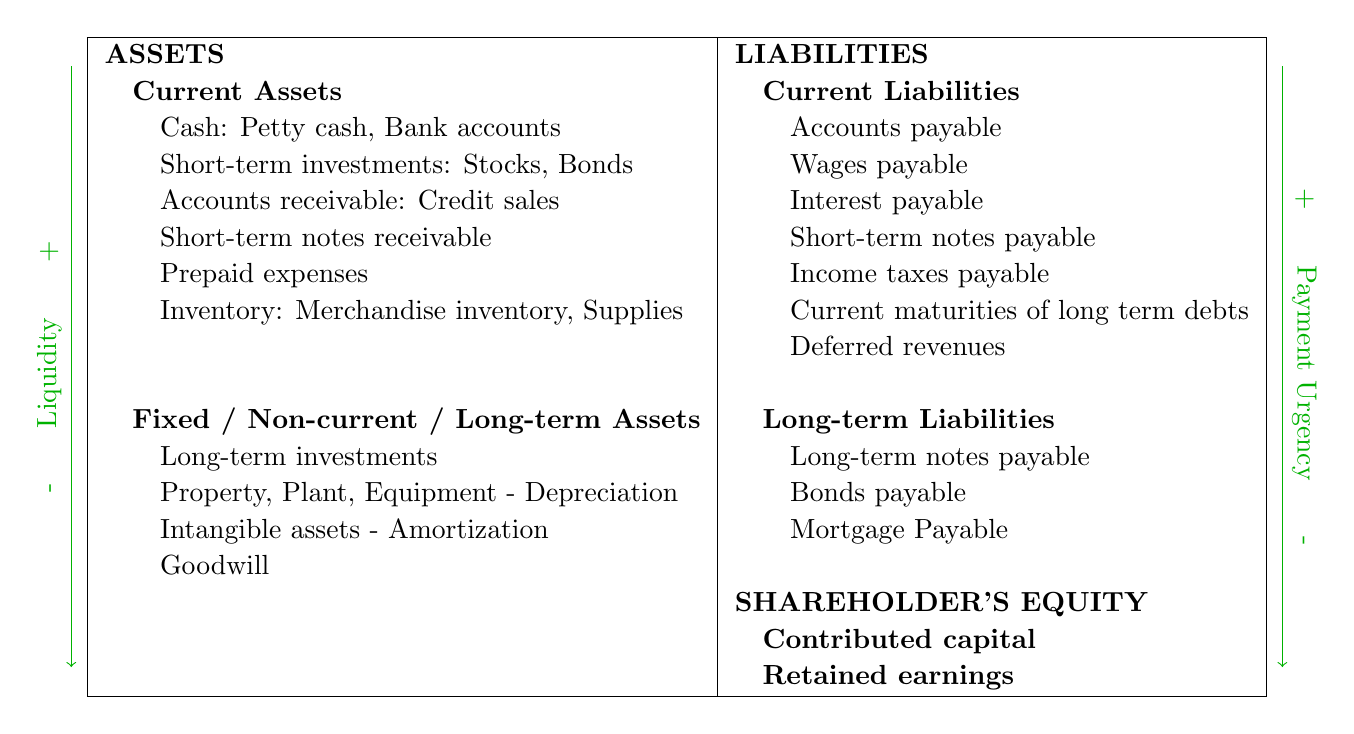
\begin{tikzpicture}
		{\renewcommand{\arraystretch}{1.1}
		\node (table) {\begin{tabular}{|l|l|}
			\hline
			\textbf{ASSETS} & \textbf{LIABILITIES} \\
			\hspace{1em}\BlueA{\textbf{Current Assets}} & \hspace{1em}\BlueA{\textbf{Current Liabilities}}\\
			\hspace{2em}Cash: Petty cash, Bank accounts & \hspace{2em}Accounts payable \\
			\hspace{2em}Short-term investments: Stocks, Bonds & \hspace{2em}Wages payable \\
			\hspace{2em}Accounts receivable: Credit sales & \hspace{2em}Interest payable \\
			\hspace{2em}Short-term notes receivable & \hspace{2em}Short-term notes payable \\
			\hspace{2em}Prepaid expenses & \hspace{2em}Income taxes payable \\
			\hspace{2em}Inventory: Merchandise inventory, Supplies & \hspace{2em}Current maturities of long term debts \\
				& \hspace{2em}Deferred revenues\\
				& \\
			\hspace{1em}\BlueA{\textbf{Fixed / Non-current / Long-term Assets}} & \hspace{1em}\BlueA{\textbf{Long-term Liabilities}}\\
			\hspace{2em}Long-term investments & \hspace{2em}Long-term notes payable\\
			\hspace{2em}Property, Plant, Equipment - Depreciation & \hspace{2em}Bonds payable\\
			\hspace{2em}Intangible assets - Amortization & \hspace{2em}Mortgage Payable\\
			\hspace{2em}Goodwill & \\
			& \textbf{SHAREHOLDER'S EQUITY} \\
			& \hspace{1em}\BlueA{\textbf{Contributed capital}}\\
			& \hspace{1em}\BlueA{\textbf{Retained earnings}}\\
			\hline
		\end{tabular}
		};
		\draw[->, green!70!black] ([xshift=-0.75mm, yshift=-5mm]table.north west) -- ([xshift=-0.75mm, yshift=5mm]table.south west) node[midway, above, rotate=90] {-\hspace{2em}\Green{Liquidity}\hspace{2em}+};
		\draw[->, green!70!black] ([xshift=0.75mm, yshift=-5mm]table.north east) -- ([xshift=0.75mm, yshift=5mm]table.south east) node[midway, above, rotate=-90] {+\hspace{2em}\Green{Payment Urgency}\hspace{2em}-};
		}
	\end{tikzpicture}
\end{center}
\vspace{-1.5mm}
The amount of highly liquid assets indicates ability to meet debt payments as they come due.
}

\subsubsectionbox{Elements of the Income Statement}{pratt2010financial,}{
\textbf{Revenues} indicate inflow of assets or reduction in liabilities, primarily from sales of 
inventories or services.
\breakspace
\textbf{COGS} or \textbf{Cost of Sales} reflects the original cost of inventory sold, either its purchase price or 
its manufacturing  cost. By subtracting this from Revenues, we arrive at the \textbf{Gross Margin}.
\breakspace
\textbf{R\&D Expenses} or Research \& Development Expenses cover costs like product innovation or supply chain 
optimizations.
Whereas \textbf{SGA Expenses} or Selling, General, and Administrative expenses, encompass costs that 
aren't directly tied to producing an item. This includes expenses such as salaries, rent, utilities, marketing,
distribution costs, customer service as well as administrative costs like office supplies, legal fees, etc.
\breakspace
By subtracting the aforementioned expenses, we derive \textbf{EBITDA}, which stands for Earnings Before Interest, 
Taxes, Depreciation, and Amortization. Further adjustments, primarily subtracting depreciation and amortization 
from EBITDA, yield the \textbf{Operating Income}, also known as \textbf{EBIT} (Earnings Before Interest and Taxes).
\breakspace
\textbf{Other revenues} (or expenses) represent minor cash inflows or outflows not related to core operations.
After accounting for these, we determine the \textbf{Net Income}, also referred to as \textbf{Profit}.
}

\subsubsectionbox{The Income Statement Visualized}{pratt2010financial, allen2017principles}{
Let's examine a scenario where better demand-supply alignment results in a 5\% sales increase, 
while also fairly accounting for a rise in costs and expenses.
\begin{figure}[H]
	\centering
	\begin{tikzpicture}[node distance=0.6mm, auto, font=\tiny]
		\def\rectheight{0.1cm}
		\tikzstyle{posRect}=[draw, rectangle, minimum height=0.20cm, fill=GreenFigA, inner sep=0pt];
		\tikzstyle{negRect}=[draw, rectangle, minimum width=0.1cm, minimum height=0.20cm, fill=RedFigA, inner sep=0pt];
		\tikzstyle{textRect}=[draw=none, rectangle, minimum height=0.20cm, align=right, inner sep=0pt];
	
		\node[posRect, minimum width=2cm] (Revenue) {};
		\node[negRect, minimum width=1.2cm, below=of Revenue.south east, anchor=north east] (COGS) {};
		\node[posRect, minimum width=0.8cm, below=of COGS.south west, anchor=north east, xshift=0.4pt] (Gross) {};
		\node[negRect, minimum width=0.1cm, below=of Gross.south east, anchor=north east, xshift=0pt] (RnD) {};
		\node[negRect, minimum width=0.3cm, below=of RnD.south west, anchor=north east, xshift=0.4pt] (SGA) {};
		\node[posRect, minimum width=0.4cm, below=of SGA.south west, anchor=north east, xshift=0.4pt] (EBITDA) {};
		\node[negRect, minimum width=0.16cm, below=of EBITDA.south east, anchor=north east, xshift=0pt] (DeprecAmort) {};
		\node[posRect, minimum width=0.24cm, below=of DeprecAmort.south west, anchor=north east, xshift=0.4pt] (OpIncome) {};
		\node[negRect, minimum width=0.02cm, below=of OpIncome.south east, anchor=north east, xshift=0pt] (Interest) {};
		\node[negRect, minimum width=0.06cm, below=of Interest.south west, anchor=north east, xshift=0.4pt] (Taxes) {};
		\node[posRect, minimum width=0.016cm, below=of Taxes.south west, anchor=north west, xshift=0pt] (Other) {};
		\node[posRect, minimum width=0.176cm, below=of Other.south east, anchor=north east, xshift=0pt] (Profit) {};

		\node[textRect, left=of Revenue.west, anchor=east, xshift=-3mm] (Revenuetext) {Revenue};
		\node[textRect, below=of Revenuetext.south east, anchor=north east] (COGStext) {COGS or Cost of Sales};
		\node[textRect, below=of COGStext.south east, anchor=north east] (Grosstext) {Gross Margin};
		\node[textRect, below=of Grosstext.south east, anchor=north east] (RnDtext) {R\&D Expenses};
		\node[textRect, below=of RnDtext.south east, anchor=north east] (SGAtext) {SGA Expenses};
		\node[textRect, below=of SGAtext.south east, anchor=north east] (EBITDAtext) {EBITDA};
		\node[textRect, below=of EBITDAtext.south east, anchor=north east] (DepAmorttext) {Depreciation, Amortization};
		\node[textRect, below=of DepAmorttext.south east, anchor=north east] (OpIncometext) {Operating Income or EBIT};
		\node[textRect, below=of OpIncometext.south east, anchor=north east] (Interesttext) {Interests};
		\node[textRect, below=of Interesttext.south east, anchor=north east] (Taxestext) {Taxes};
		\node[textRect, below=of Taxestext.south east, anchor=north east] (Othertext) {Other Revenues};
		\node[textRect, below=of Othertext.south east, anchor=north east] (NetIncometext) {Net Income};

		\node[textRect, right=of Revenue.east, anchor=west, green!70!black] {+2,000};
		\node[textRect, right=of COGS.east, anchor=west, red] {-1,200};
		\node[textRect, right=of Gross.east, anchor=west, green!70!black] {800};
		\node[textRect, right=of RnD.east, anchor=west, red] {-100};
		\node[textRect, right=of SGA.east, anchor=west, red] {-300};
		\node[textRect, right=of EBITDA.east, anchor=west, green!70!black] {400};
		\node[textRect, right=of DeprecAmort.east, anchor=west, red] {-160};
		\node[textRect, right=of OpIncome.east, anchor=west, green!70!black] {240};
		\node[textRect, right=of Interest.east, anchor=west, red] {-20};
		\node[textRect, right=of Taxes.east, anchor=west, red] {-60};
		\node[textRect, right=of Other.east, anchor=west, green!70!black] {+16};
		\node[textRect, right=of Profit.east, anchor=west, green!70!black] {176};

		\node[posRect, minimum width=2.10cm, right=of Revenue.east, anchor=west, xshift=9mm] (RevenueImp) {};
		\node[negRect, minimum width=1.20cm, below=of RevenueImp.south east, anchor=north east, xshift=0pt] (COGSImp) {};
		\node[posRect, minimum width=0.900cm, below=of COGSImp.south west, anchor=north east, xshift=0.4pt] (GrossImp) {};
		\node[negRect, minimum width=0.110cm, below=of GrossImp.south east, anchor=north east, xshift=0pt] (RnDImp) {};
		\node[negRect, minimum width=0.330cm, below=of RnDImp.south west, anchor=north east, xshift=0.4pt] (SGAImp) {};
		\node[posRect, minimum width=0.460cm, below=of SGAImp.south west, anchor=north east, xshift=0.4pt] (EBITDAimp) {};
		\node[negRect, minimum width=0.176cm, below=of EBITDAimp.south east, anchor=north east, xshift=0pt] (DeprecAmortImp) {};
		\node[posRect, minimum width=0.284cm, below=of DeprecAmortImp.south west, anchor=north east, xshift=0.4pt] (OpIncomeImp) {};
		\node[negRect, minimum width=0.0237cm, below=of OpIncomeImp.south east, anchor=north east] (InterestImp) {};
		\node[negRect, minimum width=0.071cm, below=of InterestImp.south west, anchor=north east, xshift=0.4pt] (TaxesImp) {};
		\node[posRect, minimum width=0.016cm, below=of TaxesImp.south west, anchor=north west] (OtherImp) {};
		\node[posRect, minimum width=0.2053cm, below=of OtherImp.south east, anchor=north east] (ProfitImp) {};
		
		\node[textRect, right=of RevenueImp.east, anchor=west, green!70!black] {+2,100};
		\node[textRect, right=of COGSImp.east, anchor=west, red] {-1,200};
		\node[textRect, right=of GrossImp.east, anchor=west, green!70!black] {900};
		\node[textRect, right=of RnDImp.east, anchor=west, red] {-110};
		\node[textRect, right=of SGAImp.east, anchor=west, red] {-330};
		\node[textRect, right=of EBITDAimp.east, anchor=west, green!70!black] {460};
		\node[textRect, right=of DeprecAmortImp.east, anchor=west, red] {-176};
		\node[textRect, right=of OpIncomeImp.east, anchor=west, green!70!black] {284};
		\node[textRect, right=of InterestImp.east, anchor=west, red] {-24};
		\node[textRect, right=of TaxesImp.east, anchor=west, red] {-71};
		\node[textRect, right=of OtherImp.east, anchor=west, green!70!black] {+16};
		\node[textRect, right=of ProfitImp.east, anchor=west, green!70!black] {205};

		\draw[-, line width=0.1mm, black!30!white, xshift=-0.1mm] (Revenue.north west) -- (Profit.south west);
		\draw[-, line width=0.1mm, black!30!white, xshift=-0.1mm] (RevenueImp.north west) -- (ProfitImp.south west);
		
	\end{tikzpicture}
\end{figure}
}

\subsubsectionbox{Profitable operations as a source of capital}{pratt2010financial}{
Retained earnings represent the cumulative profits a company has generated and chosen to reinvest in the business 
rather than distribute as dividends. They don't pinpoint a specific tangible asset or cash pool. 
Instead, they indicate the portion of the assets listed on the balance sheet that stems from profitable operations.

\begin{figure}[H]
	\centering
	\begin{tikzpicture}[node distance=0.3mm, auto, font=\tiny]
		\def\rectheight{0.15cm}
		\tikzstyle{prevRect}=[draw, rectangle, minimum height=\rectheight, fill=Gray, inner sep=0pt];
		\tikzstyle{textRect}=[draw=none, rectangle, minimum height=\rectheight, align=right, inner sep=0pt];
		\tikzstyle{expVar}=[draw=Yellow!10!black, rectangle, minimum height=\rectheight, xshift=-0.15mm, fill=Yellow, inner sep=0pt];
		\tikzstyle{impVar}=[draw=Green!10!black, rectangle, minimum height=\rectheight, xshift=-0.15mm, fill=GreenFigA, inner sep=0pt];
		
		% Assets
		\node[prevRect, minimum width=0.5cm] (CA1) {};
		\node[textRect, above=of CA1.north west, anchor=south west, NavyBlue] (CA) {\textbf{Current Assets}};
		\node[prevRect, minimum width=0.65cm, below=of CA1.south west, anchor=north west] (CA2) {};
		\node[prevRect, minimum width=0.75cm, below=of CA2.south west, anchor=north west] (CA3) {};
		\node[prevRect, minimum width=0.95cm, below=of CA3.south west, anchor=north west] (CA4) {};
		\node[prevRect, minimum width=0.95cm, below=of CA4.south west, anchor=north west] (CA5) {};
		\node[prevRect, minimum width=0.85cm, below=of CA5.south west, anchor=north west] (CA6) {};
		\node[textRect, below=of CA6.south west, anchor=north west, NavyBlue] (LA) {\textbf{Long-term Assets}};
		\node[prevRect, minimum width=1.60cm, below=of LA.south west, anchor=north west] (LA1) {};
		\node[prevRect, minimum width=1.75cm, below=of LA1.south west, anchor=north west] (LA2) {};
		\node[prevRect, minimum width=0.35cm, below=of LA2.south west, anchor=north west] (LA3) {};
		\node[prevRect, minimum width=0.25cm, below=of LA3.south west, anchor=north west] (LA4) {};

		% Liabilities and Equity
		\node[prevRect, minimum width=0.55cm, right=of CA1.east, anchor=west, xshift=2cm] (CL1) {};
		\node[textRect, above=of CL1.north west, anchor=south west, NavyBlue] {\textbf{Current Liabilities}};
		\node[prevRect, minimum width=0.65cm, below=of CL1.south west, anchor=north west] (CL2) {};
		\node[prevRect, minimum width=0.75cm, below=of CL2.south west, anchor=north west] (CL3) {};
		\node[prevRect, minimum width=0.75cm, below=of CL3.south west, anchor=north west] (CL4) {};
		\node[textRect, below=of CL4.south west, anchor=north west, NavyBlue] (LL) {\textbf{Long-term Liabilities}};
		\node[prevRect, minimum width=1.10cm, below=of LL.south west, anchor=north west] (LL1) {};
		\node[prevRect, minimum width=1.25cm, below=of LL1.south west, anchor=north west] (LL2) {};
		\node[prevRect, minimum width=1.35cm, below=of LL2.south west, anchor=north west] (LL3) {};
		\node[textRect, below=of LL3.south west, anchor=north west, NavyBlue] (EQ) {\textbf{Equity}};
		\node[prevRect, minimum width=1.55cm, below=of EQ.south west, anchor=north west] (EQ1) {};
		\node[prevRect, minimum width=0.65cm, below=of EQ1.south west, anchor=north west] (EQ2) {};

		% Explicit Variations: Financing and Investing
		\node[expVar, minimum width=0.10cm, right=of CA1.east, anchor=west] (EV1) {};
		\node[expVar, minimum width=0.25cm, right=of CA6.east, anchor=west] (EV2) {};
		\node[expVar, minimum width=0.25cm, right=of LA2.east, anchor=west] (EV3) {};
		\node[expVar, minimum width=0.30cm, right=of CL4.east, anchor=west] (EV4) {};
		\node[expVar, minimum width=0.30cm, right=of LL1.east, anchor=west] (EV5) {};

		\node[impVar, minimum width=0.15cm, right=of EV1.east, anchor=west] (IV1) {};
		\node[impVar, minimum width=0.20cm, right=of EV2.east, anchor=west] (IV2) {};
		\node[impVar, minimum width=0.10cm, right=of LA1.east, anchor=west] (IV3) {};
		\node[impVar, minimum width=0.45cm, right=of EQ2.east, anchor=west] (IV4) {};

		% Legend
		%\node[draw, rectangle, minimum width=]
		\node[prevRect, minimum width=0.25cm, minimum height=0.10cm,
			right=of CL1.west,anchor=west, xshift=2.25cm, yshift=-6.5mm] (LG1) {};
		\node[expVar, minimum width=0.25cm, minimum height=0.10cm,
			right=of LG1.south west, anchor=north west, xshift=-0.15mm, yshift=-1.25mm] (LG2) {};
		\node[impVar, minimum width=0.25cm, minimum height=0.10cm,
			right=of LG2.south, anchor=north, xshift=-0.15mm, yshift=-1.25mm] (LG3) {};
		\node[textRect, right=of LG1.east, anchor=west] {Last Period};
		\node[textRect, right=of LG2.east, anchor=west] (FI) {Financing and Investing};
		\node[textRect, right=of LG3.east, anchor=west] {Profitable Operations};
		\node[draw, rectangle, right=of EV5.east, anchor=west,
			minimum width=23mm, minimum height=7.5mm, xshift=7.25mm, yshift=0.95mm]{};
	\end{tikzpicture}
\end{figure}

These earnings highlight the capital sourced directly from profitable operations, distinguishing it from 
capital derived from borrowings or owner contributions.
}

\subsection{Accounting for Inventory}

\subsubsectionbox{Accounting categories of Inventory}{pratt2010financial, investopedia}{
Inventory plays a central role in accounting, reflecting a company's financial well-being and operational 
stance. It represents a major portion of a firm's assets, with its management directly affecting 
profitability and liquidity. Therefore, precise record-keeping is  required to offer stakeholders a concise 
financial perspective crucial for investment decisions.
\breakspace
Shifting our lens to manufacturing, we can delineate these specific inventory categories:
\vspace{0.75mm}
\begin{itemize}
	\item \textbf{Raw Materials:} Fundamental inputs of a manufacturing process
	\item \textbf{Work in Progress (WIP):} Inventory undergoing transformation from raw materials to final products.
	\item \textbf{Components:} Individual parts, sourced or produced, essential for final product assembly.
	\item \textbf{Finished Goods:} Fully processed products ready for sale.
\end{itemize}
\breakspace
In a broader operational context, beyond pure manufacturing, we also consider:
\vspace{0.75mm}
\begin{itemize}
	\item \textbf{Merchandise Inventory:} Ready-to-sell products acquired for resale without additional modification.
	\item \textbf{Supplies:} Operational items not for sale, such as office materials.
	\item \textbf{MRO Items:} Resources for maintenance, repair, and operations, distinct from final product materials.
\end{itemize}
}

\subsubsectionbox{The Inventory Accounting Flow/Cycle}{pratt2010financial}{
\begin{figure}[H]
	\centering
	\begin{tikzpicture}[node distance=0.4cm, auto, font=\tiny]
		\tikzstyle{Rect}=[draw, rectangle, minimum height=1.0625cm, minimum width=1.7cm, fill=none,
			rounded corners=0.25mm, inner sep=0pt, align=left];
		\tikzstyle{txt}=[anchor=north west, align=left, inner sep=0.75mm];
		% Main nodes
		\node[Rect] (acquiring) {};
		\node[txt] () at (acquiring.north west)
			{\textbf{Acquiring Inventory}\\\vspace{-1mm}\\Determine:\\\ding{223} Units to include\\\ding{223} Costs to attach};
		\node[Rect, right=of acquiring.east, anchor=west](carrying) {};
		\node[txt] () at (carrying.north west)
			{\textbf{Carrying Inventory}\\\vspace{-1mm}\\Record keeping:\\\ding{223} Perpetual system\\\ding{223} Periodic system};
		\node[Rect, right=of carrying.east, anchor=west] (costflow) {};
		\node[txt] () at (costflow.north west)
			{\textbf{Cost Flow Method}\\\vspace{-1mm}\\\ding{223} FIFO\\\ding{223} LIFO\\\ding{223} Average};
		
		\node[Rect, below= of costflow.south, anchor=north, minimum width=1cm, minimum height=0.5cm]
			(ending) {\textbf{Ending}\\\textbf{Inventory}};

		\node[Rect, right=0.65cm of costflow.east, anchor=west, minimum width=1cm, minimum height=0.5cm]
			(cogs) {\textbf{Income}\\\textbf{Statement}};
		
		\draw[-{Stealth[length=1mm]}, InfoFlow] (acquiring.east) -- (carrying.west);
		\draw[-{Stealth[length=1mm]}, InfoFlow] (carrying.east) -- ++ (0.30cm, 0cm) |- (costflow.west);
		\draw[-{Stealth[length=1mm]}, InfoFlow] (costflow.south) -- (ending.north);
		\draw[-{Stealth[length=1mm]}, InfoFlow] (ending.west) -| (carrying.south);
		\draw[-{Stealth[length=1mm]}, InfoFlow] (costflow.east) --node[above, font=\tiny] {COGS} (cogs.west);
	\end{tikzpicture}
\end{figure}
}

\subsubsectionboxEDIT{Capitalization of Inventory Costs}{pratt2010financial, taxfoundationLIFO}{
Inventories are acquired at a cost and don't generate revenues until they're sold; thus, their cost is 
capitalized. Per the matching principle, the sale revenue is matched with the inventory's cost at the time of sale.
To determine the capitalized cost, first identify the number of inventory items, then assign a cost to each item.
\breakspace
To understand the policy conversation about LIFO and FIFO, one must understand two main philosophies of 
calculating income: the pure income approach and the cash flow approach.

The income approach focuses on matching deductions for costs with the revenues they generate. For example, 
if a farm invests in a new tractor that it will use for 10 years, it should spread the deductions for that 
tractor out over the next 10 years. When applying this principle to inventories, companies should deduct 
the cost of a unit of inventory when it is sold.

The cash flow approach suggests companies should deduct their costs right when those costs are incurred. 
In the case of the farm investing in a new combine, it should deduct the full cost of the combine immediately.
When applying this principle to inventories, companies should deduct the cost of a unit of inventory when it 
is acquired. 
}

\subsubsectionboxEDIT{Units to include}{pratt2010financial}{
\textbf{General Rule:} Items intended for manufacturing, sale, or consumption should be included in a company's 
inventory only if the company has full ownership of them, meaning that it bears all associated risks and benefits.
Usually, ownership implies possession of the items, and in such cases, the units to be included in the 
inventory can be straightforwardly counted.
\breakspace
However, there are situations where ownership doesn't necessarily  mean direct possession. Two of these 
notable exceptions are: Consignments and Goods in Transit.
}

\subsubsectionbox{Consignments}{pratt2010financial}{
In a consignment arrangement, the \textit{consignor} transfers inventory to a
\textit{consignee}, such as a retailer, who physically holds and sells the items. While the consignor
retains full ownership, the consignee, after selling, keeps a service fee and remits the rest of the
proceeds to the consignor. 

\begin{figure}[H]
	\centering
	\begin{tikzpicture}[node distance=1mm, auto, font=\tiny]
		\tikzstyle{Rect}=[draw, rectangle, minimum height=0.4cm, minimum width=1cm, fill=none,
			rounded corners=0.5mm, inner sep=0pt];
		% Main nodes
		\node[Rect] (consignor) {Consignor};
		\node[Rect, minimum width=1.5cm, minimum height=0.5cm, right=1.5cm of consignor.east,
			anchor=west, align=center] (consignee) {Consignee\\(e.g retailer)};
		\node[Rect, right=1.5cm of consignee.east, anchor=west] (customer) {Customer};
		
		\draw[-{Stealth[length=1mm]}] ([yshift=0mm]consignor.east) -- 
			node[pos=0.5, above, yshift=-0.2mm, align=center, font=\tiny] {Consignment \\ inventory} 
			([yshift=0mm]consignee.west);
		\draw[-{Stealth[length=1mm]}] ([yshift=0mm]consignee.east) -- 
			node[pos=0.5, above, yshift=-0.2mm, align=left, font=\tiny] {Sales} ([yshift=0mm]customer.west);

		\draw[-{Stealth[length=1.5mm]}, MoneyFlow, line width=0.25mm] ([xshift=0mm]customer.south) -- 
			++(0,-3mm) -| node[pos=0.25, above, yshift=-0.2mm, align=left, font=\tiny]
			{Revenue 100\%} ([xshift=3mm]consignee.south);
		\draw[-{Stealth[length=1.5mm]}, MoneyFlow, line width=0.20mm] ([xshift=-3mm]consignee.south) -- 
			++(0,-3mm) -| node[pos=0.25, above, yshift=-0.2mm, align=left, font=\tiny]
			{Revenue 80\%} (consignor.south);
	\end{tikzpicture}
\end{figure}

Inventory should only be disclosed in the consignor's balance sheet.
}

\subsubsectionbox{Goods in Transit}{pratt2010financial}{
Theoretically, both a seller and a buyer should record a transaction simultaneously. However, in practice,
most sales are recorded when goods are shipped, while purchases are typically recorded upon receipt of the goods.
This method is generally acceptable, unless there are \textit{goods in transit} at the end of an accounting period.
\breakspace
To properly account for such transactions, it's essential to determine the ownership of the goods while they
are in transit. Freight shipping terms like FOB (free on board) serve this purpose. This term is commonly used 
in domestic shipping within the U.S., and should not be confused
with the FOB term from the International Commercial Terms, INCOTERMS {\sffamily\textregistered} 2020.
\begin{figure}[H]
	\centering
	\begin{tikzpicture}[node distance=0mm, auto, font=\tiny]
		\tikzstyle{Rect}=[draw=none, rectangle, minimum height=0.35cm, minimum width=0.8cm, fill=none,
			inner sep=0pt, line width=0.0005mm, xshift=0mm];
		\def\scolor{LimeGreen!65!white}
		\def\bcolor{Goldenrod!65!white}

		\node[Rect, fill=\scolor] (seller) {Seller};
		\node[Rect, right=of seller.east, anchor=west, minimum width=2.5cm, fill=\bcolor]
			(shipment) {shipment};
		\node[draw=none, inner sep=0pt, above=of shipment.north, anchor=south, align=left, yshift=2mm] (a) 
			{Both a sale and a purchase \\should be recorded};
		\node[Rect, right=of shipment.east, anchor=west, fill=\bcolor] (buyer) {Buyer};
		\node[draw=none, inner sep=0pt, left=of seller.west, anchor=east, xshift=-2mm]
			(fobship) {FOB shipping point};

		\node[Rect, below=of seller.south, anchor=north, yshift=-5mm, xshift=0.1mm, fill=\scolor]
			(seller2) {Seller};
		\node[Rect, right=of seller2.east, anchor=west, minimum width=2.5cm, fill=\scolor]
			(shipment2) {shipment};
		\node[draw=none, inner sep=0pt, above=of shipment2.south, anchor=north, align=left, yshift=-2mm] (b) 
			{Neither a sale nor a purchase \\should be recorded};
		\node[Rect, right=of shipment2.east, anchor=west, fill=\bcolor] (buyer2) {Buyer};
		\node[draw=none, inner sep=0pt] at (fobship |- seller2)
			(fobdest) {FOB destination};
		
		\draw[-, line width=0.01mm] ([yshift=-0.25mm]a.south) -- (shipment.north);
		\draw[-, line width=0.01mm] (b.north) -- (shipment2.south);
		\draw[-, line width=0.01mm] (shipment.south) -- (shipment2.north);
		\path (shipment.south west) -- (shipment2.north west)
			node[draw=none, fill=gray!3, inner sep=0pt, minimum width=4cm, midway, align=left, xshift=-5mm]
			(endofperiod) {End of the accounting period};
	\end{tikzpicture}
\end{figure}
\textbf{FOB shipping point:} The seller is responsible for the goods only to the point from which they are
	shipped.\\
\textbf{FOB destination:} The seller is responsible for the goods all the way to their destination.\\
}

\subsubsectionboxEDIT{Costs to Attach}{pratt2010financial, GPT4}{
\textbf{General Rule:} Attach all the costs required to bring inventory to a saleable condition:
\begin{itemize}
	\item Acquisition (purchased or manufactured)
	\item Shipping in (or inbound transportation)
	\item Storage 
	\item Packaging
\end{itemize}
Distribution costs $\rightarrow$ These are considered as "selling expenses", not inventory costs.
}

\subsubsectionbox{Types of Discounts}{GPT4}{

\textbf{Sales-boosting Discounts:}\\
Designed to increase sales volume, either by attracting more customers or incentivizing larger purchases.\\
Promotions, Introductory Offers, Trade Discounts, Volume or Quantity Discounts
\breakspace
\textbf{Inventory Management Discounts:}\\
Discounts used to manage stock levels, clear old inventory, or promote specific products.\\
Seasonal Discounts, Markdowns, Two-for-One (and related), Overstock Discounts, Closeout Discounts
\breakspace
\textbf{Liquidity-Improving Discounts:}\\
Discounts offered to accelerate payment, enhancing the seller's (or even the buyer's) cash flow.\\
Cash Discounts (Early Payment Discounts), Deferred Payment / Simple Trade Credit.
\breakspace
\textbf{Cost and Service Discounts:}\\
Discounts that either reduce ancillary costs or add value through supplementary services.\\
Free Shipping, Loyalty Discounts, Pick-up Incentives, Tiered Service Discounts.
}

\subsubsectionbox{Cash Discounts (Early Payment Discounts)}{allen2017principles, smith1987trade}{
They're incentives for buyers to pay invoices early, improving the seller's cash flow.
For instance, "2/10 net 30" provides a 2\% discount if payment is made within 10 days;
otherwise, the full amount is due by day 30.
\begin{figure}[H]
	\centering
	\begin{tikzpicture}[node distance=0mm, auto, font=\tiny]
		\tikzstyle{Rect}=[rectangle, minimum height=0.35 cm, inner sep=0pt];
		\node[Rect, minimum width=1.25cm, fill=Green!50] (disc) {2\% discount};
		\node[Rect, right=of disc.east, minimum width=2.5cm, fill=Red!50] (full) {Full amount};
		\node[below=of disc.south east] () {day 10};
		\node[below=of full.south east] () {day 30};
	\end{tikzpicture}
\end{figure}%
\vspace{-1.25mm}
Based on the provided terms, buyers can either capitalize on a 2\% discount by paying on day 10, often via a loan, 
or leverage the extended trade credit for 20 more days by settling on day 30. From a financial perspective, it's essential to 
balance the associated debt cost against the opportunity cost of missing the discount or paying the extra amount.\\
\vspace{2mm}
\begin{minipage}{0.5\linewidth}\centering
	\textbf{Simple interest of the opportunity cost:}
	\[ \left(\frac{0.02}{0.98}\right) \left(\frac{365}{20}\right) \approx 0.37 \]
\end{minipage}%
\begin{minipage}{0.5\linewidth}\centering
	\textbf{Compound interest of the opportunity cost:}
	\[ \left(\frac{1}{0.98}\right)^{(\nicefrac{365}{20})} - 1 \approx 0.45 \]
\end{minipage}%
\vspace{2mm}\\
Annualization helps to compare the costs and evaluate alternatives, factoring in either simple or 
compounded interest for the lost funds, based on how the business handles its money.
}

\subsubsectionboxEDIT{Inventory record keeping: Periodic and Perpetual Systems}{pratt2010financial}{
\textbf{Periodic System:}
Inventory records are updated only at specific intervals, often at the end of a month or quarter. For instance,
\textit{COGS} would be calculated considering the \textit{beginning inventory} plus the \textit{purchases}
during the period minus the \textit{ending inventory}. This approach may be chosen due to technological 
constraints or specific company policies.

\begin{figure}[H]
	\centering
	\begin{tikzpicture}[node distance=0mm, auto, font=\tiny]
		% Inventory Level
		\draw[-, line width=0.25mm]
			(0cm,0.5cm) -| (0.30,0.90) -| (0.65,0.80) -| (0.85,0.70) -| (1.00,0.40) -| (1.25,1.10) -|
			(1.45,0.70) -| (1.60,0.35) -| (2.00,1.05) -| (2.20,0.95) -| (2.40,0.90) -| (2.55,0.60) -|
			(2.80,0.90) -| (3.15,0.80) -| (3.35,0.70) -| (3.50,0.20) -| (3.75,1.00) -| (4.10,0.80) -|
			(4.30,0.70) -| (4.45,0.25) -| (4.70,1.10) -| (5.05,0.80) -| (5.25,0.70) -| (5.40,0.30) -|
			(5.85,1.00) -| (6.00,0.80) -| (6.20,0.70) -| (6.35,0.25) -| (6.60,1.10) -| (6.95,0.80) -|
			(7.15,0.70) -| (7.30,0.40) -- (7.5, 0.4);

		% 3-month periods (Quarters)
		\draw[{Circle[length=0.8mm]}-{Circle[length=0.8mm]}, NavyBlue] (0, 1.4) -- ++(1.875cm,0);
		\foreach \x in {1.875, 3.75, 5.625}{
			\draw[-{Circle[length=0.8mm]}, NavyBlue] (0 + \x cm, 1.4) -- ++(1.875cm,0);
		}

		% Inventory Reviews
		\def\yvar{-0.25cm}
		\foreach \x/\y in {1.875/0.35, 3.75/0.20, 5.625/0.30, 7.5/0.40}{
			\draw[dash pattern=on1off1, NavyBlue, line width=0.1mm]
			([xshift=-0.4mm]\x,\y) -- ([xshift=-0.4mm]\x, 1.4);
		}
		\foreach \x/\y in {0.30/0.90 , 0.65/0.80 , 0.85/0.70 , 1.00/0.40 , 1.25/1.10 ,
			1.45/0.70 , 1.60/0.35 , 2.00/1.05 , 2.20/0.95 , 2.40/0.90 , 2.55/0.60 ,
			2.80/0.90 , 3.15/0.80 , 3.35/0.70 , 3.50/0.20 , 3.75/1.00 , 4.10/0.80 ,
			4.30/0.70 , 4.45/0.25 , 4.70/1.10 , 5.05/0.80 , 5.25/0.70 , 5.40/0.30 ,
			5.85/1.00 , 6.00/0.80 , 6.20/0.70 , 6.35/0.25 , 6.60/1.10 , 6.95/0.80 ,
			7.15/0.70 , 7.30/0.40 , 7.5/ 0.4
		} {
			\draw[-{Circle[length=0.4mm]}, dash pattern=on1off1, BrickRed, line width=0.05mm]
			(\x,\y) -- (\x,\yvar);
		}
		\draw[BrickRed] (0, \yvar+0.2mm) -- (7.5, \yvar+0.25mm);

		\node[align=left] () at (3.75, 1.6) {$\textbf{COGS}_{t} = I_{t-1}+ P_{t} - I_{t}$};

	\end{tikzpicture}
\end{figure}%
\vspace{-1mm}
\textbf{Perpetual System:}
Inventory is continuously updated with each transaction. Real-time tracking is often facilitated by 
Point-of-Sale Systems or technologies such as RFID, QR codes, barcodes, and ERP systems. Additionally, 
advanced innovations like the Internet of Things, Blockchain, AI, and Automation can further enhance 
tracking precision.
}

\subsubsectionbox{COGS Allocation: FIFO, LIFO, Average Method}{pratt2010financial}{
\vspace{-1mm}
\begin{figure}[H]
	\centering
	\def\acolor{MidnightBlue!55}
	\def\bcolor{Red!60}
	\begin{tikzpicture}[
			scale=0.75, every node/.style={transform shape},
			node distance=0.2mm, auto, font=\tiny, line width=0.1mm
		]
		\tikzstyle{Rect1}=[draw, rectangle, minimum width=4mm, minimum height=4mm, inner sep=0pt];
		\tikzstyle{Rect2}=[draw, rectangle, minimum width=4mm, minimum height=6mm, inner sep=0pt];
		\tikzstyle{Rect3}=[draw, rectangle, minimum width=4mm, minimum height=8mm, inner sep=0pt];
		\tikzstyle{txt}=[draw=none, rectangle, inner sep=0pt, align=center];

		\node[Rect1, fill=\acolor] (11) {};
		\node[Rect1, right=of 11.east, anchor=west, fill=\acolor] (12) {};
		\node[Rect1, right=of 12.east, anchor=west, fill=\acolor] (13) {};

		\node[Rect2, right=1.5mm of 13.south east, anchor=south west, fill=\acolor] (21) {};
		\node[Rect2, right=of 21.east, anchor=west, fill=\acolor] (22) {};
		\node[Rect2, right=of 22.east, anchor=west, fill=\acolor] (23) {};
		\node[Rect2, right=of 23.east, anchor=west, fill=\acolor] (24) {};
		\node[Rect2, right=of 24.east, anchor=west, fill=\acolor] (25) {};
		\node[Rect2, right=of 25.east, anchor=west, fill=\bcolor] (26) {};
		\node[Rect2, right=of 26.east, anchor=west, fill=\bcolor] (27) {};
		\node[Rect2, right=of 27.east, anchor=west, fill=\bcolor] (28) {};
		\node[Rect2, right=of 28.east, anchor=west, fill=\bcolor] (29) {};
		\node[Rect2, right=of 29.east, anchor=west, fill=\bcolor] (210) {};

		\node[Rect3, right=1.5mm of 210.south east, anchor=south west, fill=\bcolor] (31) {};
		\node[Rect3, right=of 31.east, anchor=west, fill=\bcolor] (32) {};
		\node[Rect3, right=of 32.east, anchor=west, fill=\bcolor] (33) {};
		\node[Rect3, right=of 33.east, anchor=west, fill=white] (34) {};
		\node[Rect3, right=of 34.east, anchor=west, fill=white] (35) {};

		\draw[-{Stealth[length=1mm]}, line width=0.25mm, Blue]
			([yshift=1.25mm]11.north west) -- ([yshift=1.25mm]13.north east) |- 
			node[above] {First Sale 8 units} ([yshift=1.25mm]25.north east);
		\draw[-{Stealth[length=1mm]}, line width=0.25mm, Red]
			([yshift=1.25mm]26.north west) -- node[above, pos=0.6] {Second Sale 8 units}
			([yshift=1.25mm]210.north east) |- ([yshift=1.25mm]33.north east);

		\node[txt, above=1.35cm of 12.south] () {\textbf{Beginning inventory = 3}};
		\node[txt, above=1.35cm of 25.south] () {\textbf{First purchase = 10}};
		\node[txt, above=1.35cm of 33.south] () {\textbf{Second purchase = 5}};

		\node[txt, left=0.45cm of 11.north west, anchor=east] () {\textbf{FIFO:}};

		% ===========================================================================================
		\node[Rect1, below=1cm of 11.south, anchor=north, fill=white] (l11) {};
		\node[Rect1, right=of l11.east, anchor=west, fill=white] (l12) {};
		\node[Rect1, right=of l12.east, anchor=west, fill=\bcolor] (l13) {};

		\node[Rect2, right=1.5mm of l13.south east, anchor=south west, fill=\bcolor] (l21) {};
		\node[Rect2, right=of l21.east, anchor=west, fill=\bcolor] (l22) {};
		\node[Rect2, right=of l22.east, anchor=west, fill=\acolor] (l23) {};
		\node[Rect2, right=of l23.east, anchor=west, fill=\acolor] (l24) {};
		\node[Rect2, right=of l24.east, anchor=west, fill=\acolor] (l25) {};
		\node[Rect2, right=of l25.east, anchor=west, fill=\acolor] (l26) {};
		\node[Rect2, right=of l26.east, anchor=west, fill=\acolor] (l27) {};
		\node[Rect2, right=of l27.east, anchor=west, fill=\acolor] (l28) {};
		\node[Rect2, right=of l28.east, anchor=west, fill=\acolor] (l29) {};
		\node[Rect2, right=of l29.east, anchor=west, fill=\acolor] (l210) {};

		\node[Rect3, right=1.5mm of l210.south east, anchor=south west, fill=\bcolor] (l31) {};
		\node[Rect3, right=of l31.east, anchor=west, fill=\bcolor] (l32) {};
		\node[Rect3, right=of l32.east, anchor=west, fill=\bcolor] (l33) {};
		\node[Rect3, right=of l33.east, anchor=west, fill=\bcolor] (l34) {};
		\node[Rect3, right=of l34.east, anchor=west, fill=\bcolor] (l35) {};

		\draw[-{Stealth[length=1mm]}, line width=0.25mm, Blue]
			([yshift=1.25mm]l210.north east) -- node[above] {First Sale 8 units} ([yshift=1.25mm]l23.north west);
		\draw[-{Stealth[length=1mm]}, line width=0.25mm, Red]
			([yshift=1.25mm]l35.north east) -- node[above] {Second Sale 5 units} ([yshift=1.25mm]l31.north west);
		\draw[-{Stealth[length=1mm]}, line width=0.25mm, Red]
			([yshift=1.25mm]l22.north east) -| node[above] {Second Sale 3 units} ([yshift=1.25mm]l13.north east) -- 
			([yshift=1.255mm]l13.north west);

		\node[txt, left=0.45cm of l11.north west, anchor=east] () {\textbf{LIFO:}};

		% ==============================================================================================
		\node[Rect1, below=0.8cm of l12.south, anchor=north] (a1) {};
		\node[txt, left=of a1.west, anchor=east] (3x) {$\frac{3}{13}\,$};
		\node[txt, right=of a1.east, anchor=west] (plus10) {$\,+\,\frac{10}{13}$};
		\node[Rect2, right=0.675cm of a1.south east, anchor=south west] (a2) {};
		\node[txt, right=0.575cm of plus10.east, anchor=west] (equals) {$\,=$};
		\node[Rect2, right=0.5cm of a2.south east, anchor=south west,
			minimum height=5.54mm, fill=\acolor] (a3) {};

		\node[txt, right=1.25cm of equals.east, anchor=west, align=left, Blue] (afirstsale)
			{First sale \\$8$ units};
		\draw[-{Stealth[length=1mm]}, line width=0.25mm, Blue]
			([xshift=0.65cm]equals.east) -- ([xshift=-0.5mm]afirstsale.west);

		\node[Rect2, right=2.5cm of a3.south east, anchor=south west,
			minimum height=5.54mm] (a4) {};
		\def\yfix{-0.8mm}
		\node[txt, left=of a4.west, anchor=east, yshift=\yfix] (5x) {$\frac{5}{10}\,$};
		\node[txt, right=of a4.east, anchor=west, yshift=\yfix] (plus5) {$\,+\,\frac{5}{10}$};
		\node[Rect3, right=0.675cm of a4.south east, anchor=south west] (a5) {};
		\node[txt, right=0.575cm of plus5.east, anchor=west] (equals2) {$\,=$};
		\node[Rect2, right=0.5cm of a5.south east, anchor=south west,
			minimum height=6.77mm, fill=\bcolor] (a6) {};
			
		\node[txt, right=1.25cm of equals2.east, anchor=west, align=left, Red] (asecondsale)
			{Second sale \\$8$ units};
		\draw[-{Stealth[length=1mm]}, line width=0.25mm, Red]
				([xshift=0.65cm]equals2.east) -- ([xshift=-0.5mm]asecondsale.west);

		\node[txt, left=0.45cm of l11.north west, anchor=east, yshift=-1.4cm] () {\textbf{Average:}};

		\draw[-{Stealth[length=0.4mm]}, line width=0.05mm]
			([xshift=1mm, yshift=-0.5mm]a3.north east) -- ([xshift=-1mm, yshift=-0.5mm]a4.north west);

	\end{tikzpicture}
\end{figure}
}

\subsubsectionbox{COGS Computation Example}{}{
Consider the following scenario with beginning inventory $I_o$, purchases and sales during a period.
The \textcolor{NavyBlue}{perpetual} system computes COGS in each transaction and the 
\textcolor{BrickRed}{periodic} system computes COGS at the end of the whole period. Cost allocation is \textbf{LIFO}.
\begin{figure}[H]
	\centering
	\begin{tikzpicture}[node distance=2.25mm, auto, font=\tiny]
		\tikzstyle{txt}=[draw=black, line width=0.1mm, rectangle, inner sep=1.5pt, fill=none, align=left];
		\tikzset{MyArrow/.style ={-{Stealth[length=1mm]}, line width=0.1mm}}

		% Purchases and Sales
		\node[txt, draw=none, fill=none, inner sep=0pt] (purchases) {Purchases:};
		\node[txt, left=of purchases.west, anchor=east] (i0) {75 @ \dollars 12};
		\node[txt, draw=none, left=of i0.west, anchor=east] (beginning) {\textbf{$I_{o}:$}};
		\node[txt, right=of purchases.east, anchor=west] (p1) {250 @ \dollars 12};
		\node[txt, draw=none, left=of p1.north west, anchor=south east] (sales) {Sales:};
		\node[txt, right=of p1.north east, anchor=south west] (s1) {300 @ \dollars 25};
		\node[txt, right=of s1.south east, anchor=north west] (p2) {400 @ \dollars 14};
		\node[txt, right=of p2.east, anchor=west] (p3) {225 @ \dollars 16};
		\node[txt, right=of p3.north east, anchor=south west] (s2) {375 @ \dollars 26};
		
		% Perpetual LIFO
		\node[txt, draw=none, above=of s1.north, anchor=south, align=right, NavyBlue] (perpetual1)
			{250 @ \dollars 12 \\ \underline{50 @ \dollars 12} \\ \dollars 3600};
		\draw[MyArrow, NavyBlue] (p1.north) |- ([yshift=-1mm]perpetual1.north west);
		\draw[MyArrow, NavyBlue] (i0.north) |- (perpetual1.west);
		\node[txt, draw=none, above=of s2.north, anchor=south, align=right, NavyBlue] (perpetual2)
			{225 @ \dollars 16 \\ \underline{150 @ \dollars 14} \\ \dollars 5700};
		\draw[MyArrow, NavyBlue] (p3.north) |- ([yshift=-1mm]perpetual2.north west);
		\draw[MyArrow, NavyBlue] (p2.north) |- (perpetual2.west);

		% Periodic LIFO
		\node[txt, yshift=-3mm, draw=none, below=of s1.south, anchor= north, align=right, BrickRed] (periodic1)
			{225 @ \dollars 16 \\ \underline{75 @ \dollars 14} \\ \dollars 4650};
		\draw[MyArrow, BrickRed] (p3.south) |- ([yshift=-1.2mm]periodic1.north east);
		\draw[MyArrow, BrickRed] ([xshift=-0.5mm]p2.south) |- (periodic1.east);
		\node[txt, yshift=-4.5mm, draw=none, below=of s2.south, anchor= north, align=right, BrickRed] (periodic2)
			{325 @ \dollars 14 \\ \underline{50 @ \dollars 12} \\ \dollars 5150};
		\draw[MyArrow, BrickRed]
			([xshift=0.5mm]p2.south) |- ([yshift=-1.2mm]periodic2.north west);
		\draw[MyArrow, BrickRed]
			(p1.south) |- ([xshift=0.5mm, yshift=-1cm]p2.south) |- (periodic2.west);
	\end{tikzpicture}
\end{figure}%
The \textcolor{NavyBlue}{Perpetual LIFO COGS is \dollars 9300} whereas 
the \textcolor{BrickRed}{Periodic LIFO COGS is \dollars 9800}.
}

\subsection{Financial Performance}

\subsubsectionbox{Measuring Performance}{}{
Foo
}

\subsubsectionbox{The Operating Cycle}{pratt2010financial}{
The operating cycle refers to the duration it takes for a company to convert its cash outflows into 
cash inflows through its core operations.
\begin{minipage}{0.6\linewidth}\centering
	\begin{figure}[H]
		\centering
		\begin{tikzpicture}[auto, font=\tiny]
			% Path: Start the 'drawing pen' at (#1:#3) then draw an arc from #1 to #2 along the ellipse #3
			\tikzset{partial ellipse/.style args={#1:#2:#3}{insert path={+ (#1:#3) arc (#1:#2:#3)}}}
			%\draw (0,0) [very thin, gray] ellipse (2cm and 1cm); % Ellipse for reference
	
			% Nodes
			\node (oc)[align=left] at (0:0) 		{Operating Cycle};
			\node (a)[align=left] at (90:1cm) 		{Cash};
			\node (b)[align=left, NavyBlue] at (20:1.7cm) 	{Manufacture or\\Purchase};
			\node (c)[align=left] at (-20:1.7cm) 	{Inventory};
			\node (d)[align=left, NavyBlue] at (-90:1cm)		{Sale};
			\node (e)[align=left] at (-160:1.7cm)	{Accounts\\Receivable};
			\node (f)[align=left, NavyBlue] at (160:1.7cm)	{Payment};
			
			% Edges and Arcs
			\draw[-, NavyBlue] (0,0) [partial ellipse=81:51:2cm and 1cm]; % The center of the ellipse is at (0,0)
			\draw[->, InfoFlow] (0,0) [partial ellipse=25:-23:2cm and 1cm];
			\draw[-, NavyBlue] (0,0) [partial ellipse=-48:-81:2cm and 1cm];
			\draw[->, NavyBlue] (0,0) [partial ellipse=-99:-125:2cm and 1cm];
			\draw[-, NavyBlue] (0,0) [partial ellipse=-161:-205:2cm and 1cm];
			\draw[->, NavyBlue] (0,0) [partial ellipse=-225:-261:2cm and 1cm];
		\end{tikzpicture}
	\end{figure}
\end{minipage}%
\begin{minipage}{0.35\linewidth}
	\textnohyphenation{The duration of this cycle can vary based on the company type, its policies, 
	industry norms, market conditions, and the nature of its transactions.
	\vspace{2mm}\\
	Current assets are those that can be converted into cash within a company's operating cycle
	or within a year, whichever is longer.}
\end{minipage}%
\vspace{1mm}
{\centering
\textnohyphenation{
\begin{tabular}{|p{1.45cm}|p{3.1cm}|p{3.1cm}|}
	\hline
	\textbf{Factors} & \textbf{Example 1} & \textbf{Example 2} \\
	\hline
	Company Type & Local craft brewery & High-end furniture manufacturer \\
	\hline
	Company Policies & Offers extended credit terms to distributors to promote their brand & Has a strict return policy, allowing only exchanges within a short window \\
	\hline
	Industry Norms & Typically, the alcoholic beverage industry sees seasonal spikes in sales, especially during holidays & In luxury furniture, customers expect customization options, leading to longer production times \\
	\hline
	Market Conditions & Due to a recent health trend, there's a surge in demand for craft beverages with natural ingredients & The economy is in a downturn, and fewer consumers are investing in luxury goods \\
	\hline
	Nature of \newline its Transactions & Primarily engages in B2B transactions with retailers and restaurants, which often involve negotiated rates and bulk deals & Engages mainly in B2C transactions through their showroom and online store, with occasional bespoke orders from corporate clients \\
	\hline
\end{tabular}}}
}

\subsubsectionbox{Working Capital}{}{
Foo
}

\subsubsectionbox{Ratios}{}{
Foo
}

\subsubsectionbox{Inventory Turnover Revisited}{}{
Foo
}

\subsection{Cost of Capital}

\subsubsectionbox{Cost of Capital}{}{
Foo
}

\subsubsectionbox{WACC}{chopra2016scm}{
\vspace{-3mm}
\begin{align*}
	\shortintertext{
	The weighted average cost of capital uses the following formula:
	}
	\text{WACC} = \frac{E}{E+D}(R_E + \beta\cdot \text{MRP}) + \frac{D}{E+D}R_D(1-t)
\end{align*}
Let's analyze this concept. First, notice the terms $\frac{E}{D+E}$ and $\frac{D}{E+D}$;
they create a weighted measure of the individual contributions of $(R_f + \beta\cdot \text{MRP})$ and $R_b(1-t)$.
}

\subsection{Pratt: Chapters 6, 7)}

\subsubsectionbox{Why 6?}{}{
It seems traditional ratio analysis is out of date, it isn't very useful.\\
Future cash flows is a more realisitc analysis\\
Must include \textbf{The Statement of Cash Flows}
}

\subsubsectionbox{Why 7?}{}{
Inventories ---> But this will be include in the next section.
}


\sectionbox{Inventory I: Deterministic Models}

\subsection{What is Inventory and why does it matter?}

\subsubsectionbox{Accounting POV vs. Logistics/SCM POV}{}{
}

\subsubsectionbox{Logistics/SCM types of inventory}{}{
}

\subsubsectionbox{Why hold inventory?}{}{
- Cover process time \\
- Decouple process \\
- ...
}

\subsubsectionbox{Inventory decisions}{}{
}

\subsection{Inventory Models}

\subsubsectionbox{Models}{}{
Trade-offs between complexity and ease of understanding/communication/implementation.
}

\subsubsectionbox{Models for Inventory Management}{}{
- Focus on costs \\
- Focus on service level \\
- ...
}

\subsection{Inventory Costs}

\subsubsectionbox{Unit Cost: $\boldsymbol{c \to \nicefrac{\$}{\text{unit}}}$}
{kcd2023, silver2016inventory, cachon2018matching, schonsleben2022handbook}{
The cost of obtaining one unit of a SKU, either through procurement or production.
\breakspace
\textbf{For merchants}:
It's the sum of the purchase price paid to the supplier, combined with additional costs necessary 
for preparing the product for sale, such as packaging and labeling. Typically, it also incorporates 
per-unit costs related to freight transportation and material handling, like loading and unloading.
\breakspace
\textbf{For producers}:
It's the total unitary production cost. Similarly, it can also include material handling and freight
transportation costs incurred from production-related activities.
Determining the unit value in manufacturing can be more challenging  due to its intricate nature.
\breakspace
In basic inventory models, the unit cost is typically considered lot-size independent for simplicity.
However, some models account for economies of scale by incorporating discounts related to the volume of 
items purchased or produced, recognizing that unit costs can vary with lot size.
\breakspace
Typically, the unit value is derived from the company's internal accounting system, 
representing its "book value",
therefore, it may differ from what SCM/logistics specialists might consider. 
Ideally, the unit value should be determined collaboratively, taking into account the actual money 
spent on that specific SKU to prepare it for either internal or external use.
}


\subsubsectionbox{Ordering/Setup Cost: $\boldsymbol{c_t} \to \nicefrac{\$}{\text{order}}$}{}{
}

\subsubsectionbox{Cost components of holding inventory}{
	silver2016inventory, axsater2015inventory, chopra2016scm, brandimarte2000}{
They vary across companies and SKUs, but, in general, they include the
following major components, which must be incremental in nature, otherwise,
they would have been incorporated as part of the fixed ordering cost:
\breakspace
\textbf{Cost of Capital:}
Capital is allocated to either purchase or produce inventory units, 
so less inventory means more available capital for alternative investments,
each with their respective rates of return.
Given that capital can be sourced from either equity or debt,
the Weighted Average Cost of Capital [WACC] is often used here,
as it's a blended measure for both sources of inventory financing.
\breakspace
\textbf{Incremental Costs of Storage:}
Warehouse space often represents a significant expenditure, especially in prime locations. 
Handling inventory -i.e. moving, organizing within the storage space—adds to the costs. 
Periodic counting or inventory audits are essential for accuracy, but require time and resources. 
Some inventory items might also necessitate special storage conditions, 
such as refrigeration or specific humidity levels, leading to additional expenses.
\breakspace
\textbf{Costs of Depreciation:}
Inventory value can diminish over time due to several reasons. 
Perishable items may degrade, rendering them unsellable. 
As new products are introduced, older items may become obsolete, 
especially in industries with rapid innovation cycles. 
Moreover, shrinkage, resulting from items being lost, stolen, or damaged, 
further erodes the inventory's value.
}

\subsubsectionbox{Holding Cost: $\boldsymbol{c_e} \to \nicefrac{\$}{(\text{unit}\times\text{period})}$}
{kcd2023, silver2016inventory}{
\vspace{-3mm}
\begin{align*}
	\shortintertext{
	Encapsulates all costs incurred from carrying a unit of inventory for a designated period.
	We can model it as:
	}
		&c_e = rc
	\shortintertext{where the \textit{holding rate} $r$ denotes a percentage of the unit value $c$ per 
	period of demand (e.g. for 1 year). A multi-SKU company may opt for $c_{e_i} = r_{i}c_{i}$​ for each SKU $i$ or, 
	to alleviate the complexity of individual analysis, apply a uniform holding rate $r$ across all SKUs.
	Accordingly, $c_e$ has the following dimensions:}
		&\frac{\$}{\text{unit}\times\text{period}}
\end{align*}
By modeling it this way, we can evaluate the cost of keeping inventory proportionally to the amount held.
\breakspace
However, in certain scenarios, the cost of storing an item remains consistent,
regardless of its value. When we employ a singular, aggregated rate $r$,
we inadvertently allow the storage component to escalate in proportion to the item's unit value. 
A more nuanced approach would be to utilize

\[ c_e=rc+h \]

Within this framework, 
$h$ stands as a constant unitary storage fee, while $r$ is solely representative of the cost of capital and
depreciation associated with the item.
\breakspace
Furthermore, consider the scenario where storage capacity is limited; if Q exceeds this threshold, an additional
warehouse is required, incurring a fixed cost. This scenario can be modeled using a piecewise function, for instance:
\[ \text{Total Holding Cost} = \begin{cases}
	Q(rc + h) 						&,\text{for} \; Q \leq \text{threshold}\\
	Q(rc + h) + \text{Fixed Cost} 	&,\text{for} \; Q > \text{threshold}
\end{cases} \]
Given the complexity of the holding cost, it's advisable to model it in collaboration with
Finance/Accounting specialists.
}


\subsubsectionbox{Stockout/Shortage Cost: $\boldsymbol{c_s}$}{}{
Can be modeled using stockout event or units short
}

\subsubsectionbox{Coordinated Cost Estimation: Finance and SCM/Logistics}{}{
Foo
}

\subsubsectionbox{Total Cost \& Total Relevant Cost}{}{

\[ \text{TC} = \text{Purchase Cost} + \text{Ordering Cost} + \text{Holding Cost} + \text{Shortage Cost} \]

\[ TC = cD + c_{t}\frac{D}{Q} + c_{e}\frac{Q}{2} + c_{s}E[\text{Units Short}] \]

Procurement activities have influence on the Purchase Cost, while Inventory Management activities have 
influence on the other costs.
}

\subsection{EOQ: Economic Order Quantity}

\subsubsectionbox{EOQ model assumptions}{}{
\begin{itemize}
	\item Known demand $\rightarrow$ Constant
	\item Zero or Constant Lead Time
	\item Something else
\end{itemize}
\par
\Red{Checkar papers review sobre EOQ}
\breakspace
\Red{Checkar variaciones en el modelado de costos (i.e. variable holding cost, setup cost, etc.) 
en Silver, Chopra, Nahmias, etc...Hay muchas variaciones, pero incluir las mas frecuentes en los libros)}
}

\subsubsectionbox{EOQ formula derivation}{}{
\vspace{-2mm}
\begin{align*}
	\shortintertext{Since demand is deterministic, we can get rid of the Stockout Cost concept for now. So,}
		TRC(Q) &= c_{t}\frac{D}{Q} + c_{e}\frac{Q}{2} \\
	\shortintertext{From the first-order optimal condition (first derivative equals zero), we have}
		0 &= \diff{}{Q}\left(\frac{c_{t}D}{Q}\right) + \diff{}{Q}\left(\frac{c_{e}Q}{2}\right) \\
		0 &= -\frac{c_{t}D}{Q^2}+\frac{c_{e}}{2} \\
		\Aboxed{Q^{*} &= \sqrt{\frac{2c_{t}D}{c_e}}}
\end{align*}

The $EOQ$ or $Q^*$ gives the minimum $TRC$ under deterministic conditions:

\begin{figure}[H]
	\centering
	\begin{tikzpicture}
	\tikzmath{\ce=5.5; \ct=400; \D=3000; \xmax=3000; \Qopt=660; \TRCopt=3633.18;}
	\begin{axis}[1Quad, width=6cm, height=4cm, hide scale,
				ymin=0, ymax=10000, xmin=0, xmax=\xmax,
				xtick={\Qopt}, xticklabels={$Q^*$},
				ytick={\TRCopt}, yticklabels={$TRC(Q^*)$},
				restrict y to domain = 0:9500]
		% Functions
		\addplot[blue, line width=0.15mm, domain=0:\xmax]{\ct*(\D/x)};
		\addplot[red, line width=0.15mm, domain=0:\xmax]{\ce*(x/2)};
		\addplot[black, line width=0.25mm, domain=0:\xmax]{\ct*(\D/x) + \ce*(x/2)};
		% Nodes
		\node[circle,draw=black,fill=black!75,inner sep=0pt,minimum size=2pt] at (\Qopt,\TRCopt){};
		% Annotations
		\draw (\Qopt,\TRCopt)node[above, xshift=0.5mm]{\tiny Optimum};
		\draw (2500,250)node[blue, above]{\tiny Ordering/Setup Cost};
		\draw (2500,4500)node[red, above]{\tiny Holding Cost};
	\end{axis}
	\end{tikzpicture}
\end{figure}
\vspace{-2mm}
}

\subsubsectionbox{EOQ Sawtooth Plot}{}{
The optimal policy becomes ordering $Q^*$ units of inventory every $T^*$ units of time.

\begin{figure}[H]
	\centering
	\begin{tikzpicture}
		\tikzmath{\lastx = 5;}
		\begin{axis}[1Quad, width=9cm, height=3.25cm, ymin=0, ymax=1.3, xmin=0, xmax=\lastx + 0.25,
					xtick style={draw=none}, xtick={\lastx-0.5}, xticklabels={1 Year},
					ytick={0.5,1}, yticklabels={,,}
					]
			% Sawtooth
			\draw (0,0) foreach \x in {1,...,\lastx} {-- ++(0,1) -- ++(1,-1)} [blue, line width=0.2mm];
			\draw (0,0.5) -- (\lastx,0.5) [darkblue, dashed, line width=0.02mm];
			\draw [pen colour={annot_color},decorate,decoration={calligraphic brace,mirror,amplitude=5pt,raise=2pt},xshift=0pt,yshift=0pt]
			(1,0) -- (2,0) node [annot_color,midway,yshift=-12.5pt, line width=5mm] {\tiny $T^*=\frac{Q^*}{D}$};
			\draw (0,1) node[annot_color, left]{\tiny $Q^*$};
			\draw (0,0.5) node[annot_color, left]{\tiny $\frac{Q^*}{2}$};
			\draw (0.45,0.6) node[annot_color, above]{\tiny $D$};
		\end{axis}
		\end{tikzpicture}
\end{figure}

Notice that the total consumption of the last order may take place after the 1 year (unit time) period.
}

\subsubsectionbox{Sensitivity Analysis for the EOQ model}{}{
Resaltar que, pese a que algunos parametros se asumen alegremente como deterministicos, el modelo es lo suficientemente
robusto como para compensar variaciones en los mismos (e.g. demanda, costos, etc.)\\

Usar los 5 libros en ...Analisis y logistica de la produccion + otros complementos
}

\subsubsectionbox{Powers of Two Policies}{}{
}

\subsection{EOQ Extensions}

\subsubsectionbox{Lead Time $> 0$}{}{
}

\subsubsectionbox{Discounts: All units}{}{
}

\subsubsectionbox{Discounts: Incremental}{}{
}

\subsubsectionbox{Discounts: One-time}{}{
}

\subsubsectionbox{Backorders}{}{
}

\subsubsectionbox{EPQ: Economic Production Quantity}{}{
}

\subsubsectionbox{Perishability}{}{
}

\subsubsectionbox{Trade Credit}{}{
}


\sectionbox{Forecasting I}

\subsection{Demand Planning}

\subsubsectionbox{Demand Planning}{}{
}

\subsubsectionbox{Demand Forecasting}{}{
}

\subsection{Data Collection}

\subsubsectionbox{Obtaining data}{}{
}

\subsubsectionbox{Aggregated data, Aggregated forecasts}{}{
}

\subsection{Time Series}

\subsubsectionbox{Time Series Components}{}{
}

\subsubsectionbox{Decomposition}{}{
}

\subsubsectionbox{Cummulative \& Naive Forecasting}{}{
}

\subsubsectionbox{Moving Averages Forecasting}{}{
}

\subsection{Forecasting Metrics}

\subsubsectionbox{Accuracy \& Bias}{}{
}

\subsubsectionbox{Error Metrics}{}{
}

\subsection{Exponential Smoothing}

\subsubsectionbox{Simple Exponential Smoothing}{}{
}

\subsubsectionbox{Damped Trend}{}{
}

\sectionbox{Forecasting II}

\subsection{Exponential Smoothing with Seasonality}

\subsubsectionbox{Seasonality Patterns}{}{
}

\subsubsectionbox{Double Exponential Smoothing}{}{
}

\subsubsectionbox{Holt-Winter Model}{}{
}

\subsubsectionbox{Initialization of Parameters}{}{
}

\subsubsectionbox{Comments and Comparison of Models}{}{
}

\subsection{Intermittent Demand Forecasting}

\subsubsectionbox{Intermittent demand patterns and examples}{}{
}

\subsubsectionbox{Approaches}{}{
}

\subsubsectionbox{Croston's Method}{}{
}

\subsection{Regression \& Causal Analysis}

\subsubsectionbox{Explaining causes of demand phenomena}{}{
}

\subsubsectionbox{Correlation and Causation}{}{
}

\subsubsectionbox{Simple Linear Regression}{}{
}

\subsubsectionbox{Multiple Linear Regression}{}{
}

\subsection{Product Development, Marketing \& Forecasting}

\subsubsectionbox{New Products Introduction}{}{
}

\subsubsectionbox{Forecasting techniques \& Product Life Cycle}{}{
}

\subsection{AI/ML techniques for Forecasting}

\subsubsectionbox{Clustering}{}{
}

\sectionbox{Inventory II: Stochastic Models}

\subsection{Stochastic Demand}

\subsubsectionbox{Demand distribution}{}{
}

\subsubsectionbox{Expected Demand}{}{
}

\subsubsectionbox{Expected Units Short}{}{
}

\subsubsectionbox{Expected Units Sold}{}{
}

\subsection{Demand Modelling}

\subsubsectionbox{Empirical Distribution}{}{
}

\subsubsectionbox{Discrete Uniform}{}{
}

\subsubsectionbox{Poisson}{}{
}

\subsubsectionbox{Continuous Uniform}{}{
}

\subsubsectionbox{Normal}{}{
}

\subsubsectionbox{Triangle}{}{
}

\subsubsectionbox{Chi-Square Test}{}{
}

\subsection{SPIM: Single Period Inventory Models}

\subsubsectionbox{SPIM: Problem introduction}{}{
}

\subsubsectionbox{Data Table}{}{
}

\subsubsectionbox{Marginal Analysis}{}{
}

\subsubsectionbox{Salvage Value}{}{
}

\subsubsectionbox{Penalty Value}{}{
}

\subsubsectionbox{Critical Ratio}{}{
}

\subsubsectionbox{Expected Profits}{}{
}

\subsection{The Newsvendor Problem}

\subsubsectionbox{Newsvendor Problem: Introduction}{}{
NFL Jersey Problem in the MicroMasters
}

\subsubsectionbox{Unit Normal Loss Function}{}{
}

\subsubsectionbox{Newsvendor Problem: Solution}{}{
}

\subsection{The Newsvendor Problem Extensions}

\subsubsectionbox{Foo}{}{
}

\sectionbox{Inventory III: Multiple Period Inventory Models}

\subsection{Introductory Models}

\subsubsectionbox{Rescaling of Parameters}{}{
}

\subsubsectionbox{Base Stock Model}{}{
}

\subsection{Continuous Review Models}

\subsubsectionbox{$\boldsymbol{(s,Q)}$ model}{}{
}

\subsubsectionbox{$\boldsymbol{(s,S)}$ model}{}{
}

\subsection{Safety Stock: Service Cost and Metrics}

\subsubsectionbox{Cycle Service Level}{}{
}

\subsubsectionbox{Cost per Stockout Event}{}{
}

\subsubsectionbox{Item Fill Rate}{}{
}

\subsubsectionbox{Cost per Item Short}{}{
}

\subsubsectionbox{Inputted and Implied Metrics}{}{
}

\subsection{Periodic Review Models}

\subsubsectionbox{$\boldsymbol{(R,S)}$ model}{}{
}

\subsubsectionbox{$\boldsymbol{(...)}$ model}{}{
}

\sectionbox{Inventory IV: Multiple Dimension Models}

\subsection{Multiple Items}

\subsubsectionbox{Grouping}{}{
}

\subsubsectionbox{Grouping: Powers of Two}{}{
}

\subsubsectionbox{Grouping: Exchange Curves}{}{
}

\subsection{Multiple Locations}

\subsubsectionbox{Location Pooling}{}{
}

\subsection{Multiple Classes}

\subsubsectionbox{Segmentation Revisited}{}{
- Fast moving items \\
- Slow moving items \\
...
}

\subsubsectionbox{A Items}{}{
}

\subsubsectionbox{B Items}{}{
}

\subsubsectionbox{C Items}{}{
}

\subsection{Multiple Echelons}

\subsubsectionbox{Multiple Echelons}{}{
}

\sectionbox{Transportation I: Freight Transportation}

\subsection{Freight Transportation}

\subsubsectionbox{Time-Space Diagram}{}{
}

\subsubsectionbox{Packaging}{}{
- Cases \\
- Pallets \\
- Containers \\
...
}

\subsubsectionbox{Transportation Modes and Routes}{}{
	?
}

\subsection{Transportation Networks}

\subsubsectionbox{Physical Network}{}{
}

\subsubsectionbox{Operational Network}{}{
}

\subsubsectionbox{Strategic Network}{}{
}

\subsection{Transportation \& Inventory}

\subsubsectionbox{Transportation Cost Functions}{}{
}

\subsubsectionbox{Total Inventory \& Transportation Cost}{}{
}

\subsubsectionbox{Transit \& Lead Time Variability}{}{
}

\subsubsectionbox{Random Sum of Random Variables}{}{
}

\subsection{Mode Selection}

\subsubsectionbox{Foo}{}{
}

\sectionbox{Transportation II: Analysis}

\subsection{The Transportation Product}

\subsubsectionbox{Four Fundamental Operations}{}{
}

\subsubsectionbox{Loading \& Unloading}{}{
}

\subsubsectionbox{Linehaul Moves}{}{
}

\subsubsectionbox{Vehicle Routing}{}{
}

\subsubsectionbox{Facility Sorting}{}{
}

\subsection{Transportation Economies}

\subsubsectionbox{Economies of Scale}{}{
}

\subsubsectionbox{Economies of Scope}{}{
}

\subsubsectionbox{Economies of Density}{}{
}

\subsection{Transportation Economic Modes}

\subsubsectionbox{Direct Transportation}{}{
}

\subsubsectionbox{Consolidated Transportation}{}{
}

\subsection{Transportation \& Routing Problems}

\subsubsectionbox{$1:1$}{}{
}

\subsubsectionbox{$1:\infty$}{}{
}

\subsubsectionbox{$\infty:1$}{}{
}

\subsubsectionbox{$\infty:\infty$}{}{
}

\sectionbox{Warehouse Management}

\subsection{Warehousing}

\subsubsectionbox{Why warehouses?}{}{
}

\subsubsectionbox{Types of warehouses}{}{
}

\subsection{Warehousing \& Packaging}

\subsubsectionbox{Foo}{}{
}

\subsection{Core Operational Functions}

\subsubsectionbox{Receive}{}{
}

\subsubsectionbox{Put away}{}{
}

\subsubsectionbox{Store}{}{
}

\subsubsectionbox{Pick}{}{
}

\subsubsectionbox{Check, Pack, Ship}{}{
}

\subsubsectionbox{Return handling}{}{
}

\subsubsectionbox{Value-added services}{}{
}

\subsection{Layout design}

\subsubsectionbox{Foo}{}{
}


\subsection{Cross-Docking}

\subsubsectionbox{Foo}{}{
}

\subsection{Segmentation \& Benchmarking in Warehousing}

\subsubsectionbox{Foo}{}{
	\begin{figure}[H]
		\centering
		\begin{tikzpicture}
		\begin{sankeydiagram}
		\sffamily
		\sankeyset{
			ratio=1cm/10,
			outin steps=2,
			draw/.style={draw=none, line width=0.1pt},
			color/.style={fill/.style={fill=#1, fill opacity=.99}},
			shade/.style 2 args={fill/.style={left color=#1, right color=#2, fill opacity=.75}},
			% colors
			@define HTML color/.code args={#1/#2}{\definecolor{#1}{HTML}{#2}},
			@define HTML color/.list={
				cyan/a6cee3, lime/b2df8a, red/fb9a99, orange/fdbf6f,
				violet/cab2d6, yellow/ffff99, blue/1f78b4, green/33a02c
			},
		}
		\def\vdist{5mm}
		\def\hwidth{.5em}
		\def\hdist{2cm}
	
		\sankeynode{name=consignor, quantity=4}
		\sankeyadvance[color=black]{consignor}{2em}
		\sankeyfork{consignor}{1.5/consignor-to-consignee2, 2.5/consignor-to-consignee1}
	
		\sankeynode{name=consignee1, quantity=2.5, at={[xshift=3cm, yshift=-0.05cm]consignor.right}, anchor=right}
		\sankeynode{name=consignee2, quantity=1.5, at={[yshift=0.1cm]consignee1.left}, anchor=right}
		\sankeyfork{consignee1}{2.5/consignee1-from-consignor}
		\sankeyfork{consignee2}{1.5/consignee2-from-consignor}
		\sankeyadvance[color=black]{consignee1}{1.5em}
		\sankeyadvance[color=black]{consignee2}{1.5em}
		\sankeyfork{consignee1}{2.5/consignee1-to-customer}
		\sankeyfork{consignee2}{1.5/consignee2-to-customer}
	
		\sankeynode{name=customer,  quantity=4, at={[xshift=3cm, yshift=0.05cm]consignee1.right}, anchor=right}
		\sankeyfork{customer}{1.5/customer-from-consignee2, 2.5/customer-from-consignee1}
		\sankeyadvance[color=black]{customer}{2em}
			
		\sankeyoutin[shade={gray!70}{cyan!70}]{consignor-to-consignee1}{consignee1-from-consignor}
		\sankeyoutin[shade={gray!70}{green!70}]{consignor-to-consignee2}{consignee2-from-consignor}
		\sankeyoutin[shade={cyan!70}{gray!70}]{consignee1-to-customer}{customer-from-consignee1}
		\sankeyoutin[shade={green!70}{gray!70}]{consignee2-to-customer}{customer-from-consignee2}
	
		% \node[anchor=west, inner sep=.1em, font=\tiny] at (consignor) {Consignor};
		% \node[anchor=west, inner sep=.1em, font=\tiny, align=left] at (consignee) {Consignee\\(e.g. retailer)};
		% \node[anchor=west, inner sep=.1em, font=\tiny] at (customer) {Customer};
	
		\end{sankeydiagram}
		\end{tikzpicture}
	\end{figure}
}

% ===============================================================================================================
\newpage
\subsection{Templates}

\subsubsectionbox{Consequences of the Axioms}{}{
By set theory definitions we have: \boxed{A \cup A^{c} = \Omega} \, and \,  \boxed{A \cap A^{c} = \emptyset}
\bcentering{P(A) \leq 1}
$A$ and $A^{c}$ are disjoint $\then P(A \cup A^{c}) = 1 = P(A) + P(A^{c}) \then P(A^{c}) = 1 - P(A)$,
and by \textit{nonnegativity} we get $P(A^{c}) \geq 0 \then P(A) \leq 1 \qed$
\bcentering{P(\emptyset) = 0}
Let $A = \Omega \then P(\Omega) + P(\Omega^{c}) = 1 \then 1 + \emptyset = 1  \then P(\emptyset) = 0 \qed$\\
%\vspace{1.5mm}
Let $\Omega$ be a finite set and $A_{1},...,A_{n}$ be disjoint events, then:
\bcentering{P\left(\bigcup_{i=1}^{n}A_{i} \right) = \sum_{1}^{n} P(A_{i})}
$P(A \cup B \cup C)=P\left[(A \cup B) \cup C\right]$. From additivity, given that the events are disjoint, we have $(P(A) + P(B)) + P(C)$.
By induction we can extend this to $n$ disjoint sets $\qed$\\
%\vspace{2mm}
Let $\{\omega_{1},...,\omega_{k}\}$ be a discrete, finite set of sample points, then:
\bcentering{P\big(\{\omega_{1},...,\omega_{k}\}\big) \then P\left(\,\bigcup_{j=1}^{k}\{\omega_{j}\} \right) \then \sum_{j=1}^{k}P\big(\{\omega_{j}\}\big)}
because $\{\omega_{1},\dots,\omega_{k}\}$, can be seen as the union of \textit{unit sets}, and since they are disjoint, additivity applies $\!\qed$.
Although, a simpler, non rigorous notation can be used: $\sum_{j=1}^{k}P(\omega_{j})$.
}

\subsubsectionbox{More Consequences of the Axioms}{}{
Consider the condition $P(A \cap B) \geq 0, \then$ The events could be joint, therefore, more generally:\\
%\vspace{1.5mm}
{\centering
	\begin{minipage}{1.75cm}
		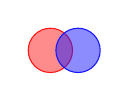
\begin{tikzpicture}
			\fill[draw=\ldraw, fill opacity=0.5, red!90!white] (0:0pt) circle (8pt);
			\fill[draw=\ldraw, fill opacity=0.5, blue!90!white] (0:10pt) circle (8pt);
		\end{tikzpicture}
	\end{minipage}%
	\begin{minipage}{4cm}
		\boxed{P(A \cup B) = P(A) + P(B) - P(A \cap B)}
	\end{minipage}
\\}
%\vspace{1.5mm}
Which can be generalized to the...:
\bcentering{P\left( \bigcup_{i=1}^{n} A_i\right) = -\sum_{k=1}^{n} (-1)^k \sum_{1 \leq i_{_1} < ... < i_{_k} \leq n} P \left( \, \bigcap_{j=1}^{k} A_{i_j} \right)}
From the above, the \textit{Union Bound} property follows: \boxed{P(A \cup B) \leq P(A) + P(B)}\\
%\vspace{1.5mm}
Consider that $A$ is included in $B$, then:\\
%\vspace{1.5mm}
{\centering
	\begin{minipage}{1.75cm}
		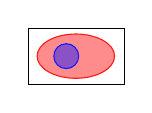
\begin{tikzpicture}
			\begin{axis}[hide axis, xmin=0, xmax=1, ymin=0, ymax=1, clip=false, width=2.8cm,height=2.3cm,]
				\fill[draw=\ldraw, fill opacity=0.5, red!90!white] (0.5,0.5) ellipse (14pt and 8pt);
				\fill[draw=\ldraw, fill opacity=0.5, blue!90!white] (0.4, 0.5) circle (4.5pt);
				\draw[line width=0.05mm] (axis cs:0,0) rectangle (axis cs:1,1);
			\end{axis}
		\end{tikzpicture}
	\end{minipage}%
	\begin{minipage}{3cm}
		\boxed{A \subset B \then P(A) \leq P(B)}
	\end{minipage}
\\}
%\vspace{1.5mm}
since $B = A \cup (B \cap A^{c}) \then P(B) = P(A) + P(B \cap A^{c}) \geq P(A) \qed$ \\  
%\vspace{1.5mm}

Consider 3 sets not necessarily disjoint, e.g.:\\
%\vspace{1.5mm}
\begin{minipage}{2cm}
	\centering
	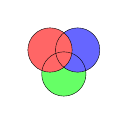
\begin{tikzpicture}
		\fill[draw=none, fill opacity=1, green!60!white] (0:0pt) circle (8pt);
		\fill[draw=none, fill opacity=1, blue!60!white] (60:10pt) circle (8pt);
		\fill[draw=none, fill opacity=1, red!60!white] (120:10pt) circle (8pt);
		\draw [draw=black, line width=0.05mm] (0:0pt) circle (8pt);
		\draw [draw=black, line width=0.05mm] (60:10pt) circle (8pt);
		\draw [draw=black, line width=0.05mm] (120:10pt) circle (8pt);
	\end{tikzpicture}
\end{minipage}%
\begin{minipage}{3cm}
	\boxed{P(A \cup B \cup C) =  \textcolor{red}{P(A)} + \textcolor{blue}{P(A^{c} \cap B)} + \textcolor{green!70!black}{P(A^{c} \cap B^{c} \cap C)}}
\end{minipage}
\\
%\vspace{1.5mm}
Visually, we can check the boxed expression by the matching of the colors, and since the subsets are disjoint, additivity holds.  Notice the expression also applies to disjoint sets $\qed$
}

\subsubsectionbox{Multiplication Rule}{}{
%\vspace{-1mm}
\begin{align*}
	\shortintertext{Notice that:}
		P(A \cap B) &= P(B) P(A|B) \\
					&= P(A) P(B|A) \\
	\shortintertext{And for 3 events we have:}
		P[(A \cap B) \cap C] &= P(A \cap B) P(C|A \cap B) \\
						   &= P(A) P(B|A) P(C|A \cap B)\\
	\shortintertext{More generally:}
		\Aboxed{P\left(\bigcap_{i=1}^{n} A_{i}\right) &= P(A_{1})\prod_{i=2}^{n}P\left(A_{i} \Bigg| \bigcap_{j=1}^{i-1} A_{j} \right)}
\end{align*}\\
A particular intersection of events would be represented as a full path in a probability tree.
}
\end{multicols*}

\newpage
\textbf{REFERENCES:}
\printbibliography

\end{document}